\documentclass[10pt,conference,final]{IEEEtran}

\usepackage[utf8]{inputenc}
\usepackage[T1]{fontenc}
\usepackage{listings}
\usepackage{color}

\usepackage{hyperref}
\usepackage{hypcap}
\usepackage{breakurl}

% für text
\usepackage{amsmath}
\usepackage[hang]{subfigure}
\usepackage{paralist}
\usepackage{ragged2e}
%\usepackage{microtype}
%\usepackage{apacite}
\usepackage{blindtext}
\usepackage{multirow}

\usepackage{siunitx}
\usepackage{footnote}
\usepackage{chngcntr}
\makesavenoteenv{tabular}
\makesavenoteenv{table}

\newcolumntype{M}[1]{>{\centering\arraybackslash}m{#1}}

\definecolor{mygreen}{rgb}{0,0.6,0}

\lstset{basicstyle=\ttfamily\footnotesize,
	breaklines=true,
	language=Java,
	keywordstyle=\color{blue},
	morekeywords={contract ,function ,if, else, public},
	commentstyle=\color{mygreen},
	tabsize=2,
	numbers=left,
	stepnumber=1,
	firstnumber=1,
	numberfirstline=true,
	xleftmargin=2.5em,
	frame=single,
	framexleftmargin=2em}

\usepackage{clrscode}
\usepackage{xcolor}
\usepackage[pdftex]{graphicx}

\newcommand{\comment}[1]{{\parindent0pt\fbox{\begin{minipage}{0.45\textwidth}{\em #1}\end{minipage}}}}
\newenvironment{changed}{\red}{\color{black}}
\newcommand{\todo}[1]{ \color{red} \footnote{ \color{red}[#1] \color{black}} \color{black}}
\newcommand{\Hide}[1]{%
 { 
   \parindent0pt
   \emph{\scriptsize #1}
 }
}
%\renewcommand{\Hide}[1]{}

\newcommand{\documenttitle}{Peer Behavior and Resilience Analysis of the Ethereum Peer--to--Peer Network}

\begin{document}

%----------------------------------------------------------------------
% Title Information, Abstract and Keywords
%----------------------------------------------------------------------
\title{\documenttitle}

% % %
% In case of double blind submissions:
%\author{
%  \IEEEauthorblockN{Anonymous}
%  \IEEEauthorblockA{Some Research Group\\
%    Some Institution\\
%    Some Email Addresses%
%  }
%}

\author{
  \IEEEauthorblockN{Anonymous}
  \IEEEauthorblockA{\\
    \\
    %
   } 
}


\maketitle


\begin{abstract}

\Hide{
Ten years ago the only really widely adopted use case for peer-to-peer (P2P) networks was filesharing.
But over these last years another application evolved and receives attention by millions of people: Blockchains.
As a consequence lots of research focused on a wide range of different aspects of blockchains but most of these target the application level, such as its cryptography, consensus protocols or smart contracts.
Only a few papers look at the underlying technology, the P2P networks and the ways how these blockchain applications utilize them.
These P2P networks build the backbone of all blockchains and therefore represent an important part in this whole construct.
To improve the security of blockchains, first of all it needs to be understood how the network and all nodes within it behave.
As previous P2P research mostly focused on filesharing networks and protocols like KAD and Overnet, we want to expand such analyses of node behavior on Ethereum, the second-largest blockchain application by market capitalization and the first one to implement a distributed execution platform.
Therefore we develop a network crawler to create snapshots of the network over a timeframe of multiple weeks.
We analyze the snapshots for node behavior and assess the resilience of the Ethereum P2P network.
Additionally we evaluate the network properties on the level of Autonomous Systems (AS).
}
\end{abstract}
\vspace{2mm}

\begin{IEEEkeywords}
% http://www.ieee.org/organizations/pubs/ani_prod/keywrd98.txt
Networks, Distributed Computing, Peer-To-Peer Computing, Security, Measurement
\end{IEEEkeywords}
% }

\maketitle

%\IEEEpeerreviewmaketitle

\section{Introduction}
Over the last few years hundreds of different blockchain protocols evolved.
Most are merely a copy of already existing protocols.
Only a few of them implement new features in comparison to the others.
Ethereum \cite{1,2} is one of these exceptions.
It's the second-largest crypto-currency by market capitalization, but strives for much more than that.
The currency ``ether'' is only the fuel for Ethereums ``world computer'', a distributed execution platform \cite{3,4}.
A neccessity to ensure rightful execution within its network.
Ethereum aims to be much more than just a blockchain.
It envisions an ecosystem for distributed and publicly verifiable execution of so-called smart contracts \cite{5}.
These smart contracts are turing-complete programs living on the blockchain.
They are invokable by any user in the network and are executed on every node to ensure their correct execution.
In addition to the capabilities of normal computer programs, smart contracts are also able to receive and manage funds in the form of ether.
With this property they represent a powerful economic asset which can handle monetary funds in predefined ways.
As ether worth many billion USD might be managed over the Ethereum blockchain, the security of the whole system is an important factor.
Many studies analyzed different aspects of the Ethereum application and protocol, like smart contract security (e.g. \cite{7,8}) or less energy consuming consensus protocols (e.g. \cite{9,10}).
But only a handful of papers discussed P2P properties of the Ethereum network (Section \ref{sec:RelatedWork}).
An important aspect for the security of the network is the behavior of the nodes.
Both the realization of attacks and the resilience of the network depend on it.

So to enable better detection and mitigation of attacks, we analyze the behavior of nodes and evaluate graph properties of the network.
To gather these information we built a crawler which collected network snapshots over a timeframe of three weeks.
We analyzed these snapshots with regards to node distribution across ASes, session length and intersession length of the found nodes and identify propably misbehaving nodes.
Further we analyzed the degree distribution of the nodes and the resilience against random failures and targeted attacks by utilizing GTNA \cite{11}, a framework to analyze the graph-theoretic properties of networks.

We organised the remainder of this paper as follows.
In section \ref{sec:BaR} we give background information to get a basic understanding of the blockchain technology and the graph-theoretic aspects we are focusing on.
Section \ref{sec:Methodology} presents our methodology divided in the crawler and the analysis of the crawled data.
In section \ref{sec:Results} we show and discuss our results and will draw a conclusion in section \ref{sec:Conclusion}.

\vspace{2mm}

\section{Background and Related Work}
\label{sec:BaR}
We want to provide the reader with sufficient background on the blockchain technology, P2P networks and the analyzed properties.
Further we discuss related work.

\vspace{2mm}

\subsection{Background}
\label{sec:Background}

\vspace{2mm}

\subsubsection{Blockchain}
\label{sec:Blockchain}
A blockchain is an append-only database which tracks state changes in the form of transactions.
In most blockchains these transactions include some kind of monetary value and in some cases also data.
Blockchains use a P2P network to be able to function without a central authority.
So the database is distributed among all nodes in the network and is maintained by the nodes themselves.
Transactions can be send by users which are represented by a cryptographic key pair.
The used scheme is the Elliptic-Curve Digital Signature Algorithm (ECDSA).
While the public key acts as receive address for transactions, the private key is used to sign and send a transaction.
With this cryptographic scheme, any user of the network can verify if a transaction is valid.
Also the private key allows access to the assets associated with the matching public key.

To allow partial ordering of transactions and weak finality, transactions are grouped into blocks which are cryptographically chained together and contain a reference of their direct predecessor.
These blocks are then synchronized between all nodes, so every participant of the network knows the current state of the blockchain.
To mitigate the double spending funds, it must be ensured that every node has the same correct state of the blokchain.
Therefore all blockchain networks implement some kind of consensus algorithm.
In most public blockchains at time of writing this is the Proof-of-Work (PoW).
By collecting transactions in blocks, only the transactions within an accepted block are considered valid.
But for a block to be accepted, it needs to fulfill some requirements.
In PoW blockchains the hash of both the block header and a nonce needs to be calculated and must be smaller than a given target.
In order to achieve this the nodes vary the nonce.
The nodes trying to find a suitable hash and create new blocks are called miners.
The target can be adjusted to reduce or increase the necessary effort to compute a valid hash value.
This adjustment is done to maintain equal times between blocks.
Without it the block time would shrink as computational power is growing constantly.
To incentivize miners to spend their computaional resources, the miner finding a block is revarded with some of the blockchains currency.
In order for miners to include transactions and not just create empty blocks, the sender of these transaction include a fee which the miners can collect for themselves.
All other nodes can validate the correctness of a block by checking the hash of the block header and verifying the signatures of all transactions within this block.

As every node should be able to mine new blocks, not only the blocks themselves but also the transactions need to be broadcasted between the nodes.
Because of network latencies, there is a small possibility for two blocks to be created simultaneously; they both are blocks of block height \(n\).
As there is only one valid block per block height allowed, the network needs to agree on one block.
To resolve this issue, the miners start their calculations on the first block they received.
When the next block is found on block height \(n + 1\), the block this one builds upon is accepted for block height \(n\).

In order to change a transaction multiple blocks ago, an attacker would have to recreate all blocks since the one containing this transaction.
But as the computational power needed to do this and catch up with the honest chain would be even larger than the one maintaining the honest chain, it is almost impossible to revert or change transactions older than a few blocks.

Ethereum combines this distributed ledger with an execution platform.
Each node has a virtual machine running, the Ethereum Virtual Machine (EVM) \cite{6}.
Additionally to normal accounts, Ethereum also has ``internally owned'' accounts which are controlled by program code.
These internally owned accounts are better known as smart contracts.
Every user can write smart contracts and create them on the blockchain via a transaction.
Afterwards the smart contract lives autonoumous on the blockchain.
Nobody can control it, despite the code of the contract allows this.
To invoke a function in the contract, a user sends a transaction to the address of it with a specific payload, so the miner processing this transaction knows what contract and what function to execute.
Besides checking transaction signatures and block hashes, all nodes should also verify the correct execution of smart contracts.
Therefore they execute the smart contract in their locally runnning instance of the EVM.
In order for a contract invocation to be executed, the user needs to send some ether to pay the miner that executes the requested action, so-called ``gas''.
Gas is not a currency, it is more a transaction internal unit to represent, how much effort the execution of a transaction takes.
The user has to pay \(gas \times gasPrice\) in ether.
So the sender has to specify both gas amount and gas price.
The amount of gas depends on the complexity of the invoked function while the gas price acts like a normal transaction fee.
Miners can choose the transactions they want to include into their block.
So the miners might want to choose only transactions whose gas price is above a certain limit, so they earn more money for the same amount of execution.
The purpose of gas is the mitigation of transaction spamming. \cite{12}

\vspace{1mm}

\subsubsection{P2P Networks}
\label{sec:P2P}
Like most other blockchain protocols, Ethereum utilizes a P2P network.
In the case of Ethereum the network communication consists of three protocols: RLPx\footnote{\url{https://github.com/ethereum/devp2p/blob/master/rlpx.md }}, DEVp2p\footnote{\url{https://github.com/ethereum/devp2p/blob/master/devp2p.md }} and the Ethereum Subprotocol.
RLPx covers the node discovery and the establishment of a secure TCP connection.
DEVp2p uses the TCP sessions to establish a session for the application layer.
The Ethereum Subprotocol handles data transfers like transaction forwarding and block synchronization.
As our work focuses on the node discovery, we will only explain the RLPx protocol.
For more extensive descriptions, please refer to \cite{13,14}.

The Ethereum RLPx protocol is based on Kademlia \cite{15}, a P2P protocol widely used in filesharing networks.
It allows efficient storage and retrieval of content over a distributed network.
In Kademlia node IDs are random 160-bit keys, while the keys of stored data result from the hash of the content and its filename.
With these IDs and keys nodes can calculate the ``distance'' between nodes and files by computing the bitwise XOR over both values.
Data is then stored on the nodes with the ``closest'' IDs.
Additionally the nodes maintain a routing table consisting of 160 buckets, each holds upto 16 node IDs and represents a different distance to other nodes.
When finding a new node, it is stored in the corresponding bucket depending on its distance to this node.
To learn the location of a file, the searching node just asks its neighbors for the file itself or the closest nodes these neighbors know for the given key.
The searching node iterates this step, until it finds a node having the file in question.

Ethereum uses a slightly different implementation of the Kademlia protocol.
The node IDs of Ethereum nodes have a length of 512 bits and also act as public keys to establish authenticated TCP sessions.
Next RLPx does not use XOR but \(\lfloor\log_{2}(a \oplus b)\rfloor\) as distance metric, where \(a\) and \(b\) are the Keccak-256 hashes of the node IDs.
Because of this altered distance there are not 160 but 256 buckets; they still hold upto 16 node IDs.
Lastly, RLPx does not support data storage and retrieval, as Ethereum is not a filesharing network, but a blockchain protocol.
The only file downloadable is the Ethereum blockchain itself which is done by the Ethereum Subprotocol.\cite{13}

The Go-Ethereum client\footnote{\url{https://github.com/ethereum/go-ethereum }} runs the node discovery routine with random IDs until it reaches its maximum peer limit (by default set to 25) and starts it again if connected nodes cancel the connection.
For bootstrapping purposes, Ethereum offers bootstrapping nodes which are hardcoded into all official Ethereum clients.

\vspace{1mm}

\subsection{Related Work}
\label{sec:RelatedWork}
Outside the blockchain space, there was already a huge amount of research done with regards to crawling P2P networks.
Most of the work focused on network properties of Overnet \cite{22,24} or KAD \cite{23,25,18}.
Kutzner et al. \cite{22} measured network statistics like network size, node availability and node distribution. by crawling the whole network for two weeks.
Bhagwan et al. \cite{24} crawled the Overnet network and analyzed different aspects of availability.
Their work has shown effects like the influence of ignoring IP aliasing or the impact of the time of day.
Steiner et al. \cite{23,25} focused on KAD and crawled it for several months.
They examined session lengths, arrival/departure and geographic distribution of nodes and found that KAD IDs are not necessarily persistent over different sessions.
Key metrics like daily availability and session length seem to be different depending of the country of origin of a peer.
Salah et al. \cite{18} also crawled the KAD network and focused on graph-theoretic properties.
They analyzed degree distribution of the nodes and the resilience of the network.

But with regards to blockchains on the P2P level, research gets sparse, except for Bitcoin \cite{26}.
It received much attention, mainly about mining strategies and vulnerabilities (\cite{27,28,29,30}), attacks against the network (\cite{31,32}) and consensus algorithms (\cite{33,34}).
Only a few papers (e.g. \cite{37,35,36}) targeted the Bitcoin P2P network, even less take a look at Ethereum \cite{13,21}.
Feld et al. \cite{36} analyzed the peer distribution of Bitcoin on the AS-level.
They show that Bitcoin is by far not as distributed as commonly thought.
They found $10,500$ nodes in $1,700$ ASes, but more than 30\% of these nodes were located in only 10 ASes.
Apostolaki et al. \cite{37} also state that Bitcoin is heavily centralized at AS-level.
Therefore it is vulnerable to BGP hijacking as no more than 100 prefixes need to be hijacked in order to partition the network.
Gencer et al. \cite{35} considered both Bitcoin and Ethereum.
They measured network statistics like bandwidth and latency.
Additionally they analyzed metrics like distribution of mining power, its utilization rate and mining fairness.
Luke et al. \cite{21} focused on multiple aspects of Ethereum.
They analyzed the Ethereum network for smart contract transactions, their lifetime and some security aspects.
Also did they crawl the network to learn about the size of the network, IP and geographical distribution.
Kim et al. \cite{13} on the other hand develop an Ethereum crawler called NodeFinder focusing on client characteristics.
They exemplify the heterogenity of the network nodes by analyzing their client software and version, client age and the supported protocols.
With regards to the network they measure peer latency and network size.

\vspace{2mm}

\section{Methodology}
\label{sec:Methodology}
As our goal was to create continuous snapshots of the Ethereum network, our first step was to learn more about the Ethereum network.
At the moment of writing there are no publicly available and accurate sources for the number of nodes in its network.
Websites like Ethernodes\footnote{\url{https://ethernodes.org }} and Etherscan\footnote{\url{https://etherscan.io/nodetracker }} give rough estimations.
However both sources show a difference of almost one thousand nodes as Ethernodes states $8,601$ nodes while Etherscan offers only $7,635$ nodes on February 6th 2019.
So we assume a vague network size of about nine thousand nodes.

Our second step was to write a crawler capable of finding as many nodes in the network in the shortest time possible.
As \cite{38} discussed, the accuracy of captured snapshots is directly dependent on the speed of the crawler and the duration of the crawl.
The slower the crawler finds nodes while using the same duration, the less nodes will be discovered, obviously.
But as there are always nodes entering and leaving the network, the longer a crawl lasts, the snapshots will contain nodes which are not any longer online and find other nodes which came online only recently.
The longer the duration of the crawl is, the less accurate the snapshot will become.
Therefore it is essential for our crawler to be fast so the necessary duration to crawl the whole network is as low as possible.

\vspace{2mm}

\subsection{Crawler}
\label{sec:Crawler}
As base we chose the official Go-Ethereum client\footnote{\url{https://github.com/ethereum/go-ethereum }} (Geth, based on Golang\footnote{\url{https://golang.org }}) version 1.8.19 which remains compatible with all current version of the used protocols.
In order to get the Geth client to crawl the network, we had to implement a few changes.
We disabled block synchronization and transaction forwarding.
Further did we change the dicovery procedure.

In unmodified state of the Geth client the discovery interval is set to four seconds.
Following this interval, the client starts a \texttt{lookup} function to search for a random node ID.
This is done to fill the buckets of the routing table.
As we want to find nodes with our crawler, this function is part of our solution.
We use this \texttt{lookup} function as entry point for our crawler.
Instead of searching random IDs, we start multiple go-routines.
Each of these routines receives an ID prefix for which it should start the search.
The routines send \texttt{findnode} calls to the $16$ closest nodes to the target IDs the routines are looking for.
Each responding node will give $16$ nodes they know of back to the routines.
The routines add these $16$ nodes to their queue of nodes that have to be asked.
Each routine maintains a map of IDs it has already asked for, so these will be skipped if they appear in their queue.
For each node in the queue the routines send a \texttt{PING} to it to learn if this node is online.
As the used UDP protocol is connectionless, we cannot be certain that a node is not reachable, if we receive no \texttt{PONG} message.
Therefore if there was no answer from the node, the routine sends a second \texttt{PING}.
This allows for a higher probability to receive an answer even with a stressed network connection.
If the node was reachable, a \texttt{findnode} call will be send.
The received nodes are again added to the queue.
All nodes that answered our \texttt{PING} messages are pushed into a single channel.
In parallel another routine gathers all the nodes from this channel and places them in a map to avoid duplicates.
This map contains the node ID, IP, UDP port, and a map of connected node IDs.

As each of the searching routines maintains its own queue and map of already asked nodes, it is possible that routines ask the same node.
What might seem like redundant work, is actually useful for our case.
Each routine asks its nodes for another target ID.
Because of that, the answers the same node sends to the routines differ.
Therefore we will learn other connections of this node.

In contrast to KAD, where the goal of a lookup is to locate a file and download it, there is no real goal for the search for an ID.
If we don't implement a break condition, our routines will search for new nodes until they find no new nodes.
But each routine will do this on its own, so each routine would have to find no new nodes in order for it to stop.
As this would take a lot of time, we have to stop the routines at some point.
The simplest solution is to set a maximum duration a routine is allowed to run.

Without time target our crawler runs for almost an hour and the number of found nodes converged towards $9,080$ nodes\footnote{This number and the numbers from Ethernodes and Etherscan in the last section where taken on February 6th. For comparison we did also make a measurement on March 9th: Ethernodes: $8,518$, Etherscan: $8,255$, our crawler: $8,846$. As both ours and the number of Ethernodes descreased and the number of Etherscan increased, but still lies under the other values, we assume the total number of nodes in the Ethereum network to have decreased over the last month. Etherscan might have improved their crawler.}.
As this is even more than the number of Ethernodes, we assume this to be close to the real number of nodes in the Ethereum network.

Stutzbach et al. \cite{38} define \(\delta = \delta_{-} + \delta_{+}\) to be the sum of newly found nodes and missing nodes in the direct comparison of two consecutive snapshots.
At some point during the crawl this \(\delta\) will not decrease much anymore while the number of found nodes will hardly increase either.
This ``sweet spot'' needs to be found.
As we cannot compute this \(\delta\) on the fly, we did multiple test runs.
Therefore we tested different values for our time target to evaluate the most useful strategy.
Table \ref{tab:1} shows our results\footnote{This evaluation took place in the beginning of February. Hence it is not comparable with the node numbers of other dates as the network size changes constantly. Furthermore did we not list the time targets themselves as these are not expressive for the reader.}.

\begin{table}[!t]
\renewcommand{\arraystretch}{1.3}
\begin{tabular}{M{0.13\textwidth} | M{0.13\textwidth} | M{0.13\textwidth}}
Found nodes & Percentage & Time taken \\ \hline
8000 & 88.1\% & 9m14s \\
8100 & 89.2\% & 9m39s \\
8200 & 90.3\% & 10m12s \\
8300 & 91.4\% & 11m2s \\
8400 & 92.5\% & 12m21s \\
8500 & 93.6\% & 14m13s \\
8600 & 94.7\% & 16m43s \\
8700 & 95.8\% & 19m30s \\
8800 & 96.9\% & 22m47s \\
8900 & 98.0\% & 27m42s \\
9000 & 99.1\% & 32m51s \\
\end{tabular}
\caption{The time taken to find specific amounts of nodes out of 9080 nodes.}
\label{tab:1}
\end{table}

We decided to use the settings to achive a crawl in $14$ minutes and $13$ seconds.
This decision will always be a tradeoff between number of nodes and duration.
But as a growing duration will introduce a much lower accuracy, we accept $8500$ nodes as a sufficiently high amount of nodes (\textasciitilde\(93.6\%\)), while the time differences are not growing too fast yet.

As $14$ minutes is a rather long time for a network crawl, we did a short exemplary evaluation of session lengths to learn if the session lengths are long enough that a crawl duration of this length is acceptable.
Therefore we first collected a test set of nodes by crawling one prefix every minute for thirty minutes continuously.
We then had a set of $208$ nodes in our test set.
For these nodes we checked their availability over a timeframe of $1190$ minutes (\textasciitilde$19.8$h) every minute.
We again used the above mentioned technique of sending two \texttt{PING} messages, if the first one was not successful.
$166$ nodes were answering every request, which is \textasciitilde$79.8$\% of the nodes.
Another $23$ nodes were answering $1170$ or more times ($98.3$\% of the time), which results in about $11.1$\%.
And yet another $9$ nodes were answering $990$ or more times ($83.2$\% of the time), which is \textasciitilde$4.3$\%.
These nodes were not offline for a longer time period but rather answered not all our \texttt{PING} messages.
Their time being offline never exceeded $5$ minutes.
All these nodes together make up \textasciitilde$95$\% of the watched nodes.
One node was answering in an alternating way; almost every second try the node was not answering.
This might be a sign of an overloaded node.
It receives too many requests and therefore cannot answer them all.

Only the remaining 9 nodes went offline at some point within the selected timeframe, but none of them went online again.
As we did not watch for IPs but rather for the node IDs at this point, it might be that the nodes went online again with another node ID.
Before these nodes went offline, their sessions were also really long.
One of them was 60 minutes online, a handful of nodes were online for about $400-600$ minutes before going offline.

Our interpretation of this evaluation is the following.
We assume the session lengths of Ethereum nodes to be much higher on average than the session lengths of filesharing networks like KAD.
Many of the nodes are running 24/7 and go only rarely offline.
These nodes might be miners or some kind of service providers like trading platforms.
They most likely will shut down their nodes only for maintainance reasons and will start them afterwards again.
There are also a few nodes coming online for only a short timeframe\footnote{``Short'' in this context means several minutes upto a few hours.}.
Maybe they want to synchronize their copy of the blockchain or send transactions.

As this short evaluation shows, it can be assumed to be sufficient to have a crawling duration of $14$ minutes as almost all node sessions will last much longer than that.
So we setup the crawler to crawl for $14$ minutes.
As we were interested in more than single snapshots, we configured the crawler to run the crawling process every hour.
In order to gather a sufficient amount of snapshots, we crawled the Ethereum network over three weeks.
Hence we collected a set of $504$ snapshots.

\vspace{2mm}

\subsection{Analysis}
\label{sec:Analysis}
The snapshots created by our crawler were processed to form adjacency lists as representation of the network graphs, because we used GTNA to evaluate some of the graph-theoretic properties.
We define a graph \(G = (V,E)\), where \(V\) represents the set of vertices, i.e. the nodes of the Ethereum network, and \(E\) is the set of edges between two vertices, i.e. the connections between nodes.
Similar to \cite{18} we consider a directed graph where \(e_{i,j}\) is the entry in the routing table of node \(i\) pointing towards node \(j\).

For our analysis we considered two different types of graphs.
One containing all nodes which where online and responded to our messages at the time of crawling and one graph on the AS-level (See Section \ref{sec:AAS}).
Because nodes located behind a NAT are not directly addressable by our crawler, we exclude them from our snapshots.
As they are not considered part of the overlay network \cite{41}, this restriction is acceptable.
In the analysis of our network graphs we want to analyze multiple properties as they are explained in the following sections.

\vspace{2mm}

\subsubsection{Distribution over Autonomous Systems}
\label{sec:AAS}
A part of our goal is to analyze the graph-theoretic properties of the Ethereum network on the AS-level.
We want to evaluate if the foundings of \cite{36} also hold for Ethereum.
Therefore we enriched the network snapshots with information from the GeoLite 2 ASN database\footnote{Available at \url{https://dev.maxmind.com/geoip/geoip2/geolite2/ }.}.
With this database we retrieve for a specific IP the AS it is belonging to.
From the enriched snapshots we create snapshots on the AS-level by grouping all nodes which belong to the same AS together collapsing their connections.
So if there is a node \(A\) in AS \(\mathcal{A}\) and there is a node \(B\) in AS \(\mathcal{B}\), in the AS graph will be a connection between AS \(\mathcal{A}\) and AS \(\mathcal{B}\).
As we now have a graph on the AS-level we can analyse it further with regards to degree distribution and resilience.

\vspace{1mm}

\subsubsection{Degree distribution}
\label{sec:ADegree}
For both graph types we constructed, we can now analyse the degree distribution.
The degree of a node \(i\) is the sum of all routing table entries \(e_{i,j}\) (i.e. the out-degree) of node \(i\) and all routing table entries \(e_{j,i}\) of other nodes \(j\) pointing to the node \(i\) (i.e. the in-degree).

The degree distribution helps to understand the structure of a network and is used to calculate the resilience.
Further we can take a look at common degrees and evaluate the existence of hubs.

As the routines of our crawler ask for 16 connections of a node and each node might be asked by multiple routines, most nodes will answer by sending all entries of a certain bucket.
Therefore we expect many nodes with a multiple of the bucket size as out-degree.
On the other hand, the in-degree is not bound to specific values, hence the degree distribution will be spread much wider.

\vspace{1mm}

\subsubsection{Resilience of the network}
\label{sec:AResilience}
For resilience we facilitate the definition by \cite{18}:
The resilience can be considered as the fraction of the nodes that have to be removed in order to break the graph down so that no giant connected component remains.
Meaning that each of the still connected parts contains less than half of the remaining nodes in the network.
The removal depends on a removal strategy \(R\).
For our study we focused on the resilience against failures of single nodes and targeted attacks.
As \cite{18} suggests, we assume random removal as a good model for failures and removal of the nodes with the highest degree as a reasonable model for targeted attacks against the nodes with the highest degree.

Cohen et al. \cite{39} have shown that the resilience against random failures of scale-free graphs is rather high and increasing with the number of nodes in the network.
On the other hand, they \cite{40} also evaluated the resilience against targeted attacks for scale-free graphs which is quite low.
Hence we assume that the Ethereum network will have a high resilience against random failures, but won't be as resilient against targeted attacks.
For both resilience measurements we expect the values of the Ethereum network to be lower than e.g. the resilience of the KAD network measured by Salah et al. \cite{18} as the Ethereum network has a much lower number of nodes.

\vspace{1mm}

\subsubsection{Session and intersession length}
\label{sec:ASessions}
The session length stands for the duration a node is censecutively online, while the intersession length indicates the time between two sessions.
Therefore we analyze the average session lengths and intersession lengths over the three weeks we crawled the network.
We compare the averages of session lengths for all nodes and for the nodes of the same AS.

\vspace{1mm}

\subsubsection{Existence of misbehaving nodes}
\label{sec:AMisbehavior}
As last point for our analysis, we want to search for out standing nodes.
Nodes which use the same ID as others or multiple nodes on the same IP or subnet.
Nodes which might be part of an attack against the network, like sybil attacks \cite{16} or eclipse attacks \cite{17}.
Therefore we analyze our snapshots and group nodes by their /16 and /24 subnet respectively and look for subnets with huge amounts of nodes.
We label them as ``sybils'' as these nodes \emph{might} be used for a sybil attack against the network.
Additionally we compare the 16-bit prefixes of the node IDs.
We again group same prefixes together and count the apperances per prefix.
These nodes are then labeled as ``eclipses''.

\vspace{1mm}

\section{Results}
\label{sec:Results}
In this section we want to present our results with regards to the analysis aspects we described in Section \ref{sec:Analysis}.

\vspace{2mm}

\subsubsection{Distribution over Autonomous Systems}
\label{sec:RAS}
While we found a varying number of ASes over the course of our analysis, for all snapshots the amount lies between $570$ and $600$ distinct ASes.
But over all snapshots we found a total number of $1,240$ distinct ASes.
Exemplary we show the distribution of the nodes over the biggest $15$ ASes on February 15th at 0:00pm CET in Figure 1.
As there are more than $550$ other ASes, this distribution has a very long tail with $531$ ASes (or $90.6$\%) containing less than 10 nodes each and $306$ ASes (or $52.2$\%) holding only one node.
On average did we crawl $8,561$ nodes per snapshot.
Out of these, $4,760$ nodes (\textasciitilde$55.8$\%) belonged to only 5 ASes which is less than one percent of all ASes.
\cite{36} claimed that only 10 ASes contained more that 30\% of all routable nodes.
But with our findings we showed that Ethereum is by far more centralized on the AS-level than Bitcoin.

\begin{figure}[!t]
\label{fig:1}
\centering
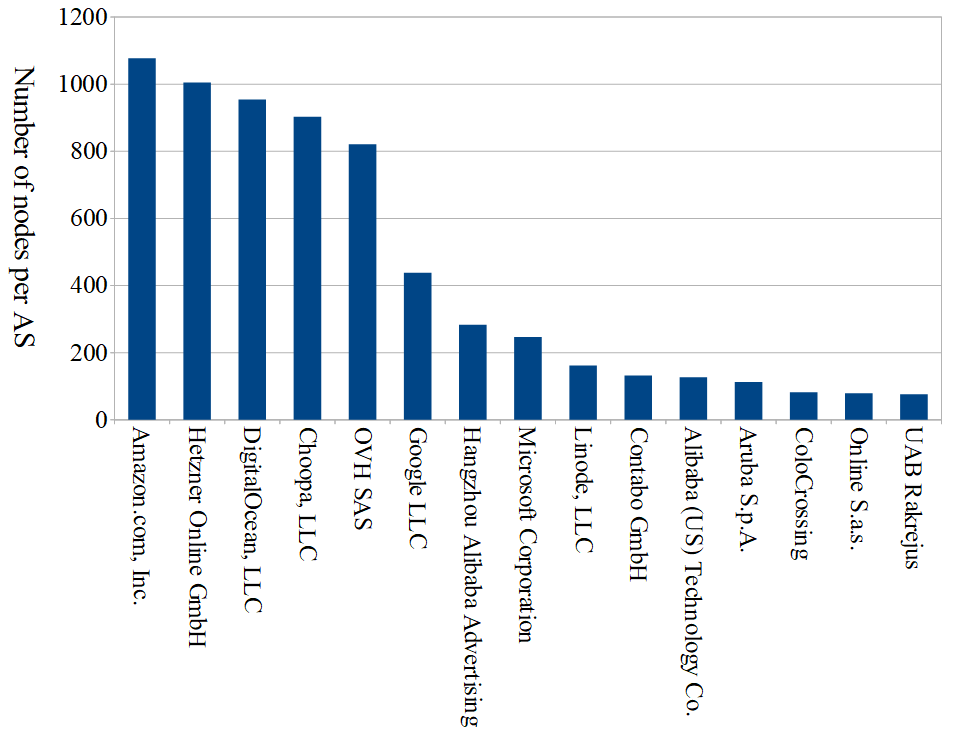
\includegraphics[width=0.49\textwidth]{./Pictures/ASdistribution.png}
%[natwidth=924,natheight=509]
\caption{Node distribution over the top 15 ASes out of 586. Example snapshot of February 15th, 0:00pm CET.}
\end{figure}

\begin{figure}[!t]
\label{fig:2}
\centering
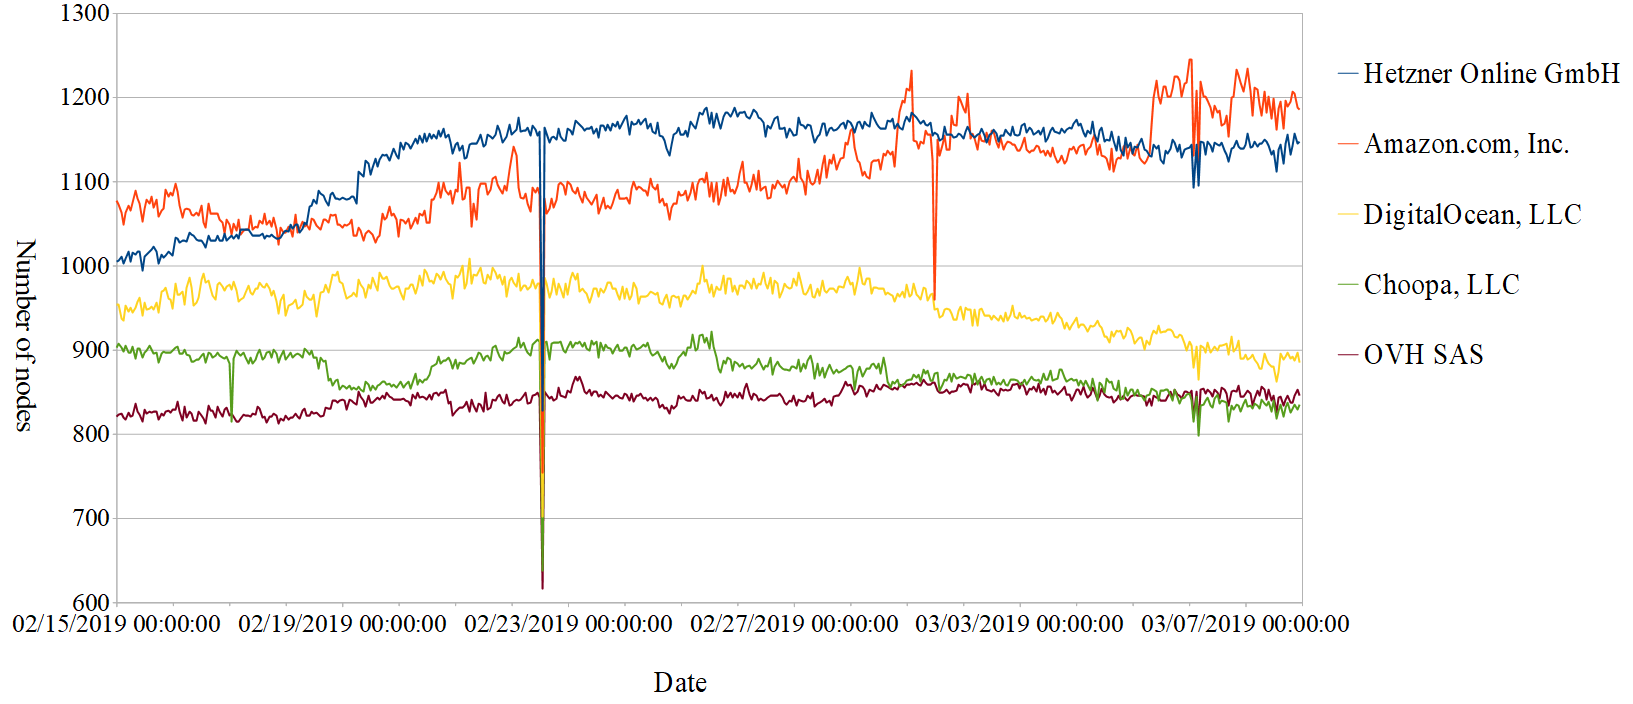
\includegraphics[width=0.49\textwidth]{./Pictures/ASdistribution1.png}
%[natwidth=924,natheight=509]
\caption{Number of nodes online in the five biggest ASes over the three weeks of crawling.}
\end{figure}

As we gathered snapshots of three weeks continuously, Figure 2 shows the fluctuation of nodes of the five biggest ASes.
We assume the spike on February 22nd to be the result of a connection issue of our crawler.
It would be a huge coincidence that over $2,500$ nodes from different ASes and different countries would be offline at the exact same time and come online again afterwards.
For the spike on the March 1st, we assume this to not be related to our network connection, as the only AS affected is ``Amazon.com, Inc.''.
Therefore it is more likely that it was a problem only occuring for this specific AS.

\vspace{1mm}

\subsubsection{Degree distribution}
\label{sec:RDegree}
Figure 3 shows the degree distribution of the nodes which where online at the time of crawling.
The total degree of the nodes seems to follow a power law.
We see many nodes with a degree below two hundred while there are only few nodes with higher degrees.
Nonetheless we found nodes with degrees of $533$, $617$ and $669$.
So there are a few hubs with hundreds of known connections.
While the wide distribution of nodes with moderate degree strengthen the overall resilience of the network, these hubs will decrease the resilience against targeted attacks as they will disrupt big parts of the network.

\begin{figure}[!t]
\label{fig:3}
\centering
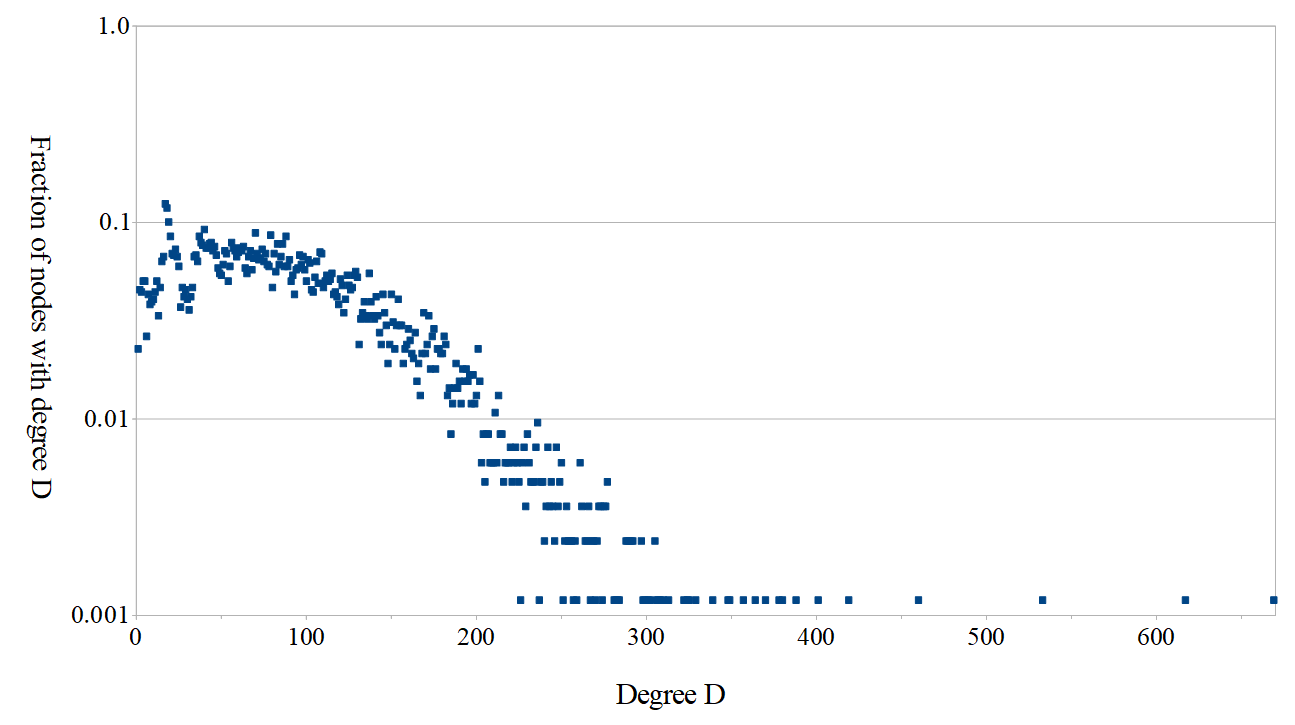
\includegraphics[width=0.49\textwidth]{./Pictures/degreeDistribution.png}
%[natwidth=924,natheight=509]
\caption{Degree distribution of the online graph. Example snapshot of February 15th, 0:00pm CET.}
\end{figure}

We also differenciated between in- and out-degree.
In Fig. 4 we show the distribution of the in- and out-degree of the online nodes.
Here we see that the out-degree indeed has high spikes at the multiple of the bucket size ($16$).
Most of the nodes have an out-degree well below one hundred.

The in-degree distribution is obviously a power law distribution with a very long tail.
And many nodes have an in-degree upto two hundred connections.
Still there are a few hubs with well over two hundred nodes, which hence are valuable targets for attacks.

\begin{figure}[!t]
\label{fig:4}
\centering
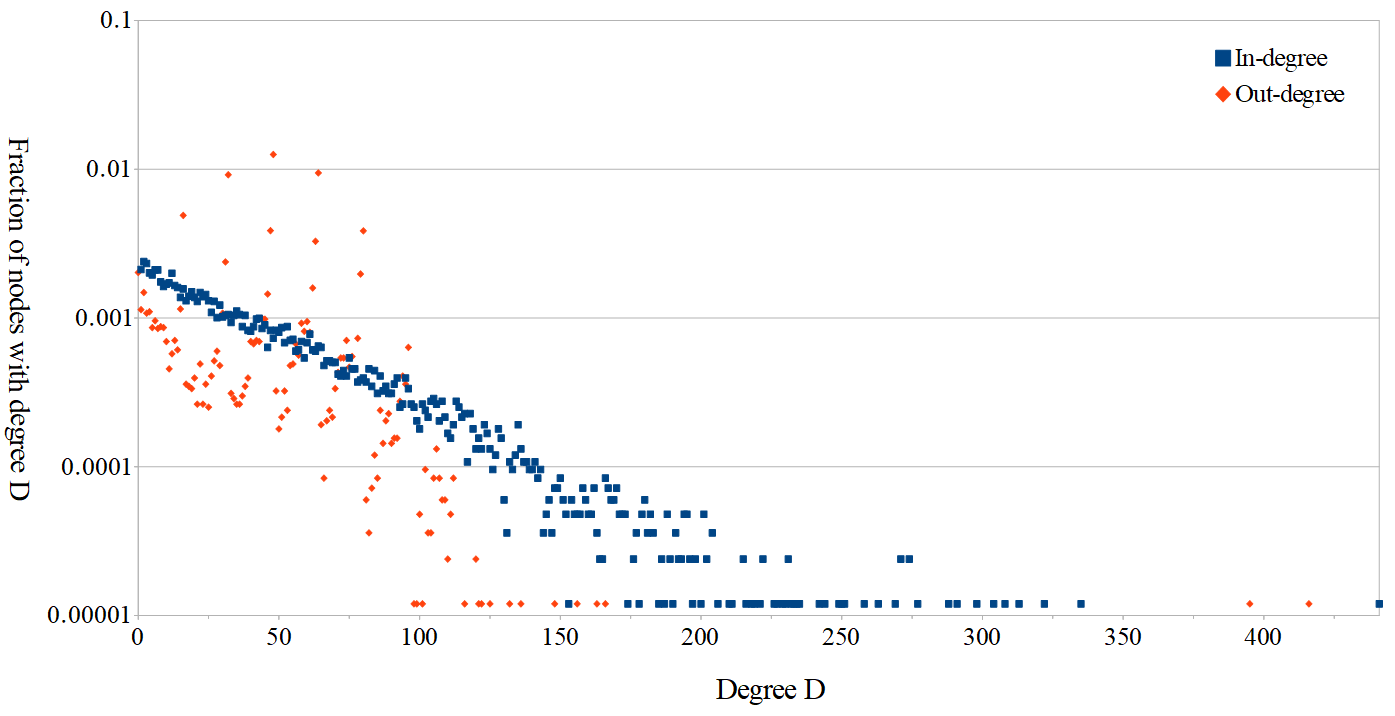
\includegraphics[width=0.49\textwidth]{./Pictures/inOutDegreeDistribution.png}
%[natwidth=924,natheight=509]
\caption{In- and out-degree distribution of the online graph. Example snapshot of February 15th, 0:00pm CET.}
\end{figure}

Every graph we generated was analyzed with GTNA.
So for each of the snapshots we additionally gathered information about the minimum, median, average and maximum for the total degree, in- and out-degree.
Over all our snapshots we calculated the average\footnote{As all snapshots are somewhat similar, we assumed, the average would be just as fine as the median.}.
We did this for both the graph of online nodes and our AS-level graph.
The results for all snapshots for the three weeks we analyzed is shown in Table \ref{tab:2}.

\begin{table}[!t]
\renewcommand{\arraystretch}{1.3}
\begin{tabular}{p{0.04\textwidth} | M{0.07\textwidth} | M{0.06\textwidth}  M{0.05\textwidth}  M{0.06\textwidth}  M{0.06\textwidth}}
 & & Minimum & Median & Average & Maximum \\ \hline
\multirow{3}{0pt}{Online \\ graph} & degree & 0.9940 & 75.1488 & 84.8135 & 652.6964 \\
 & in-degree & 0.6726 & 30.0714 & 42.4068 & 454.2381 \\
 & out-degree & 0.0000 & 46.1131 & 42.4068 & 374.0000 \\ \hline
\multirow{3}{0pt}{AS-level} & degree & 2.4107 & 38.6667 & 73.5282 & 1031.3392 \\
 & in-degree & 0.3274 & 17.8750 & 36.7641 & 547.9345 \\
 & out-degree & 1.0000 & 20.7500 & 36.7641 & 492.1667 \\
\end{tabular}
\caption{The average values of 504 snapshots for minimum, median, average and maximum values for total degree, in-degree and out-degree.}
\label{tab:2}
\end{table}

\vspace{1mm}

\subsubsection{Resilience of the network}
\label{sec:RResilience}
Further did we analyze the resilience of the Ethereum network.
We again analyzed each snapshot on its own and want to give a concluding overview.
In Table \ref{tab:3} we list the minimal, average and maximal resilience we found in all graphs for both the resilience against random failures and targeted attacks.

\begin{table}[!t]
\renewcommand{\arraystretch}{1.3}
\begin{tabular}{p{0.05\textwidth} | M{0.08\textwidth} | M{0.07\textwidth}  M{0.08\textwidth}  M{0.08\textwidth}  M{0.08\textwidth}}
 & & Minimum &  Average & Maximum \\ \hline
\multirow{2}{0pt}{Online \\ graph} & random & 0.9668 & 0.9820 & 0.9833 \\
 & targeted & 0.6468 & 0.7014 & 0.7172 \\ \hline
\multirow{2}{0pt}{AS-level} & random & 0.9912 & 0.9932 & 0.9934 \\
 & targeted & 0.5477 & 0.6393 & 0.6690 \\
\end{tabular}
\caption{The minimum, average and maximum values for the resilience of the Ethereum network.}
\label{tab:3}
\end{table}

As we expected the resilience against random failures is with about \(98.2\%\) on average quite high.
But compared to the results of \cite{18} the Ethereum network is of course not as resilient as the KAD network, but also has a much lower number of nodes.
Salah et al. crawled an average number of \textasciitilde$450,000$ nodes, while the Ethereum network only has upto $9,000$ concurrently active nodes.
The resilience against random failures is only a bit lower, but for targeted attacks the resilience is a lot worse\footnote{From the results in \cite{18} we can only compare to the values for the active graph as we only analyzed the graph of online (and therefore active) nodes.}.

When evaluating the AS-level graph, we see that the resilience against random failures is even higher than in the online graph.
On the other hand the resilience against targeted attacks is worse then the one of the online graph.
As the distribution of nodes per AS is a power law, we assume there is only a small number of ASes which build the backbone of the network.
As long as not all of them are removed (i.e. in the case of random removal) the network stays intact.
But when targeting those large ASes, the network can be distroyed quite easily.

We want to note, that we calculated the resilience of the AS-level graph the same way we did for the online graph.
Therefore when removing one AS from the graph, its numerical significance to the network is rather low despite the fact it may contain hundreds of nodes.
The number of nodes it comprises is not considered in the current form of resilience calculation.
For future work it might be interesting to adjust the calculation of resilience.
Besides the degree of the AS also the amount of nodes taken down with it should be considered.

\vspace{1mm}

\subsubsection{Session and inter session length}
\label{sec:RSessions}
Over the three weeks of crawling we found a total number of $29,654$ distinct online nodes in the Ethereum network.
For all those nodes we measured the session lengths and intersession lengths.
The average session length of all nodes lies at $30.40$ hours, while the average intersession length amounts to $69.93$ hours.
So on average each node is only about a third of the time online.

To refer to Section \ref{sec:RAS}, we show in Figure 5 the average session lengths of the nodes of all ASes with more than 100 nodes.
The number of nodes refers to all distinct nodes found over the course of the three weeks.

In Figure 6 we show the session and intersession length distribution for all (inter-) sessions we identified.
For better understanding we give the cumulative values for this distribution in Table \ref{tab:4}.
It shows, that 14.1\% of all sessions lasted longer that 24 hours.
And 6.3\% of the sessions were longer than a week.
Steiner et al. \cite{23} reported only about 0.1\% of the sessions they captured for KAD nodes to be longer than one week.
As we assumed in Section \ref{sec:Crawler}, Ethereum nodes seem to be online for a much longer duration than nodes of the KAD network.

\begin{figure}[!t]
\label{fig:5}
\centering
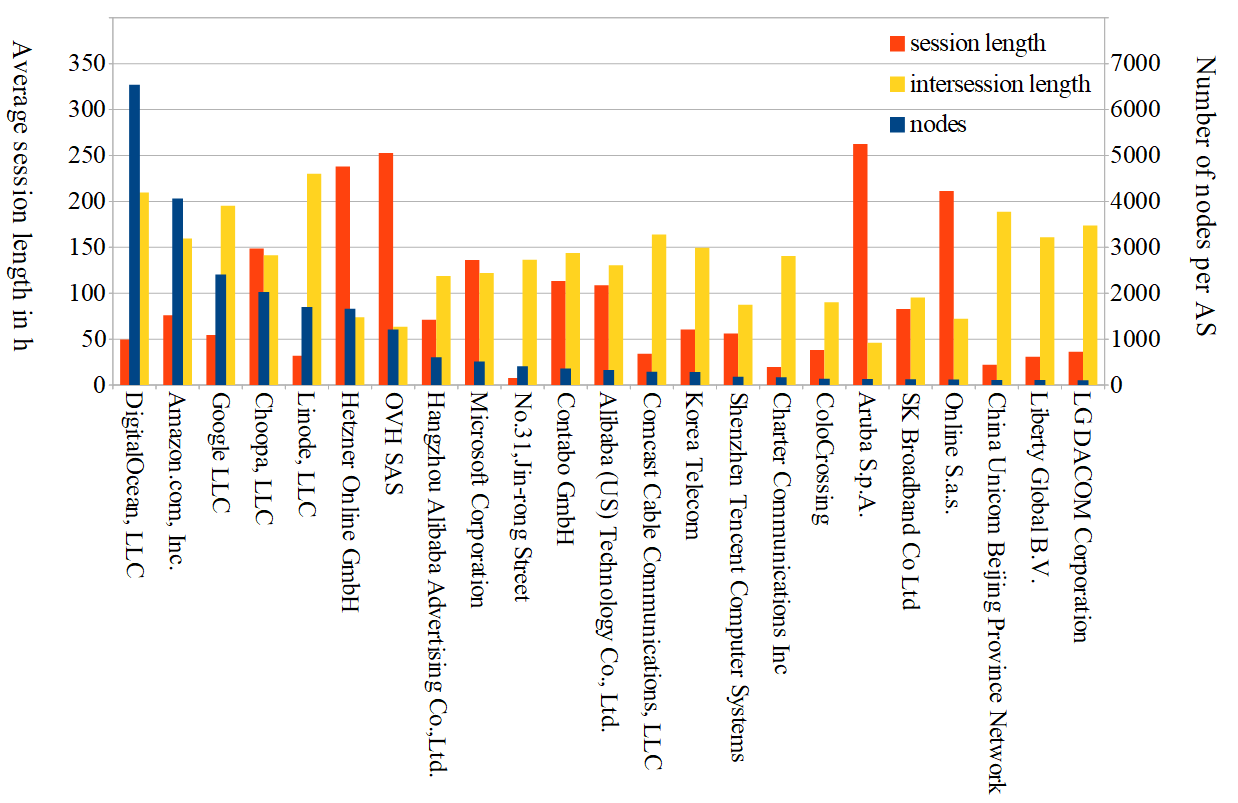
\includegraphics[width=0.49\textwidth]{./Pictures/sessionsAS.png}
%[natwidth=924,natheight=509]
\caption{Session lengths and intersession lengths of found nodes over the three weeks of crawling categorized by AS. We only consider ASes with more than 100 distinct nodes.}
\end{figure}

\begin{figure}[!t]
\label{fig:6}
\centering
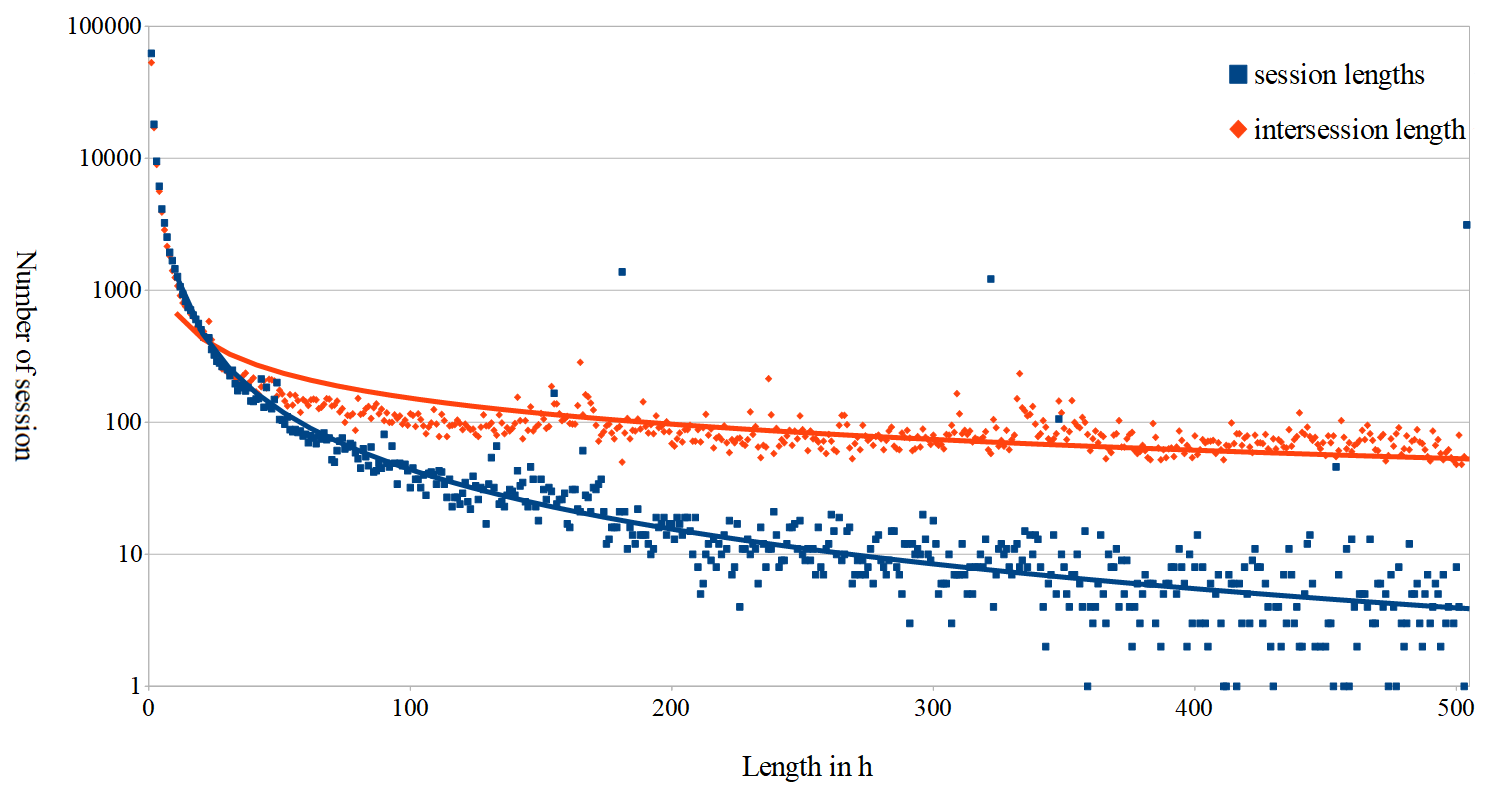
\includegraphics[width=0.49\textwidth]{./Pictures/sessions.png}
%[natwidth=924,natheight=509]
\caption{Session lengths and intersession lengths of all sessions recorded over the three weeks of crawling.}
\end{figure}

\begin{table}[!t]
\renewcommand{\arraystretch}{1.3}
\begin{tabular}{M{0.17\textwidth} | M{0.13\textwidth} | M{0.13\textwidth}}
Session duration & Number of sessions & Percentage \\ \hline
1 day & 19765 & 14.1\% \\
2 days & 14781 & 10.6\% \\
3 days & 12643 & 9.0\% \\
7 days & 8799 & 6.3\% \\
14 days & 4183 & 3.0\% \\
21 days & 3135 & 2.2\% \\
\end{tabular}
\caption{Cumulative values for number of sessions exceeding specific lengths.}
\label{tab:4}
\end{table}

\begin{table}[!t]
\renewcommand{\arraystretch}{1.3}
\begin{tabular}{M{0.25\textwidth} | M{0.18\textwidth}}
Session length & Number of occurences \\ \hline
155h (6 days, 11 hours) & 166 \\
181h (7 days, 13 hours) & 1379 \\
322h (13 days, 10 hours) & 1218 \\
348h (14 days, 12 hours) & 106 \\
504h (21 days) & 3135 \\
\end{tabular}
\caption{Specific spikes of the session length distribution.}
\label{tab:5}
\end{table}

Both lengths follow a power law.
The same session lengths are higher than the intersession lengths for durations of upto twenty hours.
From this threshold on, the intersession length occur by far more often.
On the other hand the session lengths contain a few really high spikes.
The most outstanding spikes are located around the mark of one and two weeks respectively.
Table \ref{tab:5} shows those spikes in detail.

To put these common session lengths into context, we refer the reader to Figure 2.
We assume, these spikes are results of our connection issues on February 22nd which resulted in about one thousand nodes to not be found by our crawler and the issues of the ``Amazon.com, Inc.'' AS on March 1st which is accountable for roughly one hundred nodes.
Those numbers correspond to the numbers in Table \ref{tab:5}.

The spike at a session length of 504 hours shows that many nodes ($3135$, about $37.1$\% of the network) were online the whole time of our measurements.
As we guess these nodes will stay online for long and will go offline only for short periods for maintainance, these nodes shape the backbone of the Ethereum network.
Also is the average session length rather long, hence the underlying P2P systems is quite robust.

\vspace{1mm}

\subsubsection{Existence of misbehaving nodes}
\label{sec:RMisbehavior}
As the Ethereum network is an open network and it's easy to join, there is a probability that not all nodes act honest.
Especially as the Ethereum network as crypto-platform handles billions of USD per day.
In order to get a feeling for dishonest nodes, we analyze the network for possible sybil and eclipse attacks.

A threat to most open P2P networks is the sybil attack.
The attacker creates a huge amount of distinct identities within the network.
As many honest nodes connect to the attackers nodes, she gains increasingly more power over the network.
She therefore controls big parts of the network and can decide what information are visible to other nodes.
In crypto-currencies this can lead to lost transactions, parts of the network mining on different blocks or the attacker gathering mining power in an island she controls.

In order to find such sybils we searched all snapshots for nodes coming from the same /16 subnet and classify them further into their corresponding /24 subnet.
To present our data in an appicable format, we only provide a short overview in Table \ref{tab:6}.
For our measurements we collected all /24 subnets with at least two nodes and put them together for their corresponding /16 subnet.
Therefore the minimum of nodes per /24 subnet is 2 and not 1, despite the fact that there were many signle nodes from distinct subnets.
Following from that, the median and average also ignore single nodes.
In the case of the maximum occurence of 348 nodes in a /16 subnet, these were running within 35 distinct /24 subnets all located in Finland.
Most of these subnets were rather small, two or three nodes each.
But six of these /24 subnets held 273 nodes, while one of them was running $101$ nodes from 10 distinct IPs.

\begin{table}[!t]
\renewcommand{\arraystretch}{1.3}
\begin{tabular}{M{0.12\textwidth} | M{0.1\textwidth} | M{0.1\textwidth} | M{0.07\textwidth}}
 & sybils /16 subnet & sybils /24 subnet & eclipse \\ \hline
Occurences & 93.38 & 490.84 & 574.34 \\
Minimum & 4 & 2 & 2 \\
Median & 10 & 2 & 2 \\
Average & 20.10 & 3.82 & 2.09 \\
Maximum & 348 & 110 & 9 \\
\end{tabular}
\caption{The average number of sybils/eclipses per snapshot and the minimum, median, average and maximum values for sybils per /16 and /24 network and eclipse with the same ID.}
\label{tab:6}
\end{table}

As the number of /16 subnets is not absurdly high, it was to be expected that there would be some occurences of multiple nodes coming from the same subnet.
But if there are a lot of nodes coming from the same subnet, this might be an indication of a sybil attack.
Therefore, if there were no sybil attacks, we would assume a power law distribution of occurences of nodes within the same subnet with a rather short tail.
In Figure 7 we show the distribution of such potential sybils.
This distribution looks a bit like a power law, but we found the tail to be quite long and also rather thick.
For comparison, we provide this distribution also in logarithmic scale in Figure 8.
All ``sybil'' occurences above 150 nodes per network summed up, result in $268,042$ node occurences.
As we found $8,561$ nodes on average and created $504$ snapshot, we crawled a total of about $4,315,000$ node occurences.
So the fraction of ``sybil nodes'' out of all nodes lies at 6.21\%.
We assess this fraction to be too high to not consider a sybil attack.

Related to the sybil attack is the eclipse attack.
The attacker creates a high amount of identities which are all ``close''\footnote{With regards to the networks distance metric.} around the victim.
As the victim will most likely connect to close nodes, he will end up with many or all connections to the attacker.
In a crypto-currency the attacker can control the view of the target and therefore can abuse the mining power of the victim or can perform double-sending on him. \cite{19}
In Ethereum, nodes do not have to replicate specific content on only a few nodes as KAD nodes do.
Therefore the nodes do not need to connect to close neighbors, but rather connect to random nodes.
Hence this attack is harder to implement, but also possible \cite{20}.

Nonetheless did we also analyze our snapshots for occurences of multiple nodes with a common prefix.
But as Table \ref{tab:6} shows, there is only a relatively small number of nodes with the same prefix.
In the case of the maximum of 9 nodes, all of these nodes had the same ID and were running from two different IPs.
It would be nearly impossible to create a node with the exact same ID, so we assume, the key file of the node was copied after creation and all instances on both IPs are run by the same entity.
As normal Ethereum clients have a maximum number of 25 parallel connections, these ``eclipse'' nodes would not be sufficient to perform an attack.


\begin{figure}[!t]
\label{fig:7}
\centering
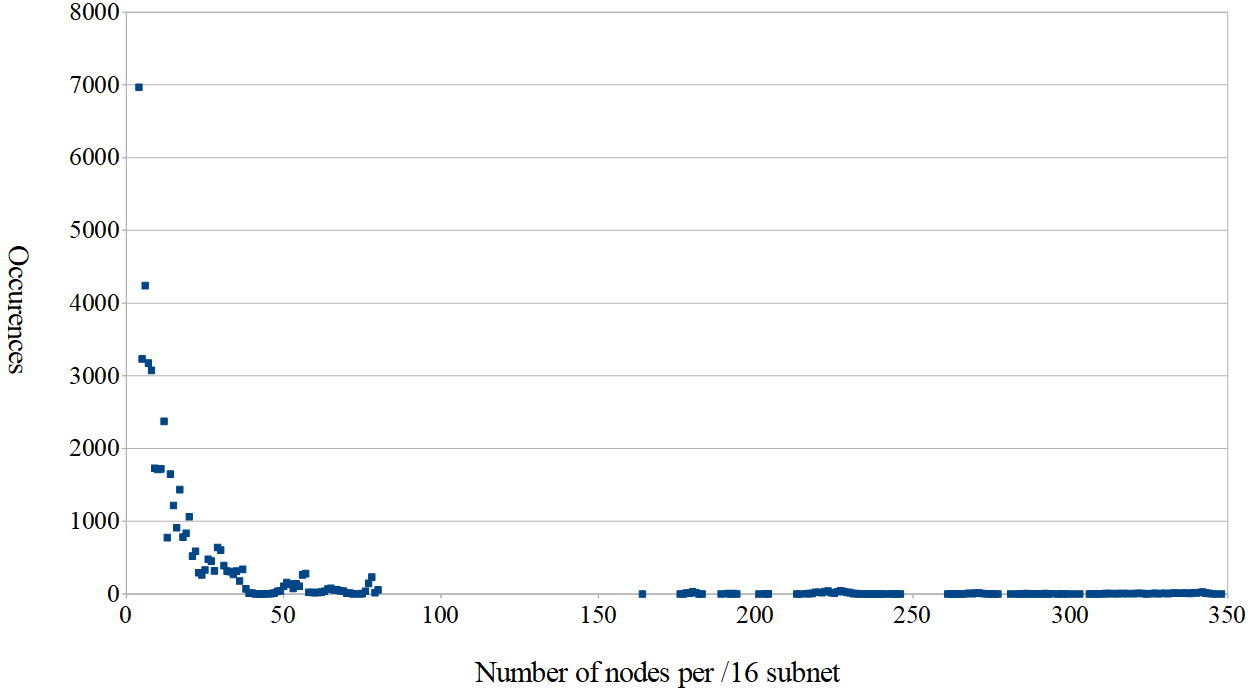
\includegraphics[width=0.49\textwidth]{./Pictures/sybils1.png}
%[natwidth=924,natheight=509]
\caption{Distribution of occurences of multiple nodes coming from the same \/16 subnet.}
\end{figure}

\begin{figure}[!t]
\label{fig:8}
\centering
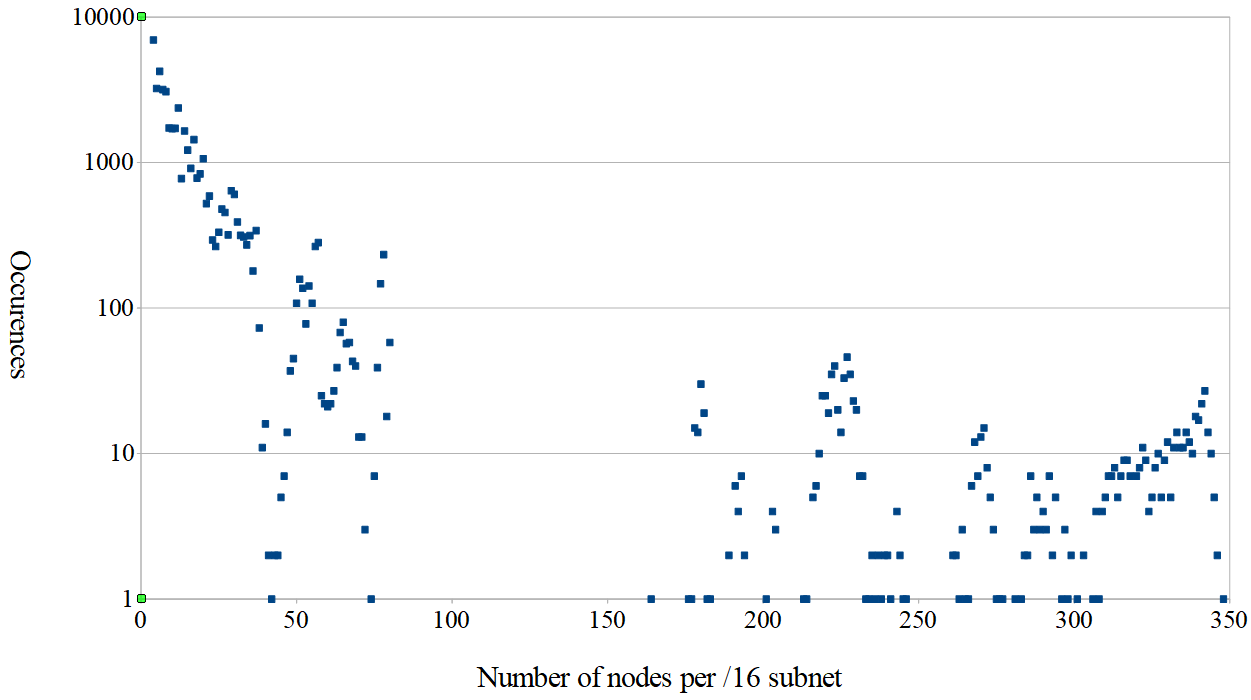
\includegraphics[width=0.49\textwidth]{./Pictures/sybils2.png}
%[natwidth=924,natheight=509]
\caption{Distribution of occurences of multiple nodes coming from the same \/16 subnet in logarithmic scale.}
\end{figure}

\vspace{2mm}

\section{Conclusion}
\label{sec:Conclusion}
The key features of P2P networks are their decentralization and robustness.
For crypto-currencies these properties are at least as important as in other distributed systems.
Recent work has already analyzed the Bitcoin network but for Ethereums P2P network none evaluated these key properties sufficiently.

In this work we implemented a crawler capable of crawling the Ethereum network in an acceptable time.
While analyzing the created snapshots, we found some rather intersting properties.
With our work we showed that the Ethereum network is on the AS-level by far not as decentralized as common sense would assume.
More than half of all nodes belong to a set of only five ASes which is even worse than the Bitcoin network as evaluated in \cite{35}.
For the degree distribution in the Ethereum network we did not find anything outstanding.
The out-degree shows high spikes at the multiples of the bucket size which is a result of the routing mechanisms used in Ethereum.
Nodes do not need to locate specific content, hence they do a lot less lookups than in a filesharing network.
Therefore they just populate the first few buckets which results in rather low out-degrees and concentrations at the multiples of the bucket size.
The in-degree follows a power law distribution as was also reported for KAD by \cite{18}.

Further did we analyze the resilience against random failures and targeted attacks.
Our results show that both measurements are below the resilience of KAD \cite{18} which is obviously a result of the much lower number of online nodes.
As there exists a good amount of hubs the resilience against targeted attacks is really low with 70.1\% on average while the resilience against random failures is acceptable with 98.2\%.
We found a high number of stable nodes being online for multiple weeks without interruption while the average session lengths is also really high in comparison to filesharing networks like KAD \cite{23}.

As for the existence of misbehaving nodes we found quite interesting numbers for possible sybils.
For /16 subnets we found upto 348 nodes, while 101 where coming from 10 distinct IPS within the same /24 subnet.
With regards to eclipse attacks we did not find any indication for a running attack.

As the Ethereum network is still not a sufficiently mature P2P network, we hope to see the network grow and gain a wider adoption.
We encourage further research on the Ethereum network as this would also support this platform to mature.








\bibliographystyle{IEEEtran}
\begin{thebibliography}{99}
\bibitem{1}
Buterin, Vitalik. ``Ethereum: A next-generation smart contract and decentralized application platform.'' \emph{\url{https://github.com/ethereum/wiki/wiki/White-Paper }} (2014).
\bibitem{2}
Wood, Gavin. ``Ethereum: A secure decentralised generalised transaction ledger.'' \emph{Ethereum Project Yellow Paper 151} (2014).
\bibitem{3}
Ethereum Foundation. 2017. What is Ether. Retrieved March 8, 2019 from \url{https://www.ethereum.org/ether }
\bibitem{4}
Taylor Gerring. 2017. What is Ethereum. Retrieved March 8, 2019 from \url{https://github.com/ethereum/wiki/wiki/What-is-Ethereum }
\bibitem{5}
Szabo, Nick. ``The idea of smart contracts.'' \emph{Nick Szabo's Papers and Concise Tutorials} (1997).
\bibitem{6}
Buntinx, JP. ``What is the Ethereum Virtual Machine?'' \emph{The Merkle}. Retrieved March 8, 2019 from \url{https://themerkle.com/what-is-the-ethereum-virtual-machine/ }
\bibitem{7}
Luu, Loi, et al. ``Making smart contracts smarter.'' \emph{Proceedings of the 2016 ACM SIGSAC Conference on Computer and Communications Security}. ACM, 2016.
\bibitem{8}
Atzei, Nicola, Massimo Bartoletti, and Tiziana Cimoli. ``A Survey of Attacks on Ethereum Smart Contracts (SoK).'' \emph{International Conference on Principles of Security and Trust}. Springer, Berlin, Heidelberg, 2017.
\bibitem{9}
Saleh, Fahad. ``Blockchain without waste: Proof-of-stake.'' (2018).
\bibitem{10}
Gervais, Arthur, et al. ``On the security and performance of proof of work blockchains.'' \emph{Proceedings of the 2016 ACM SIGSAC Conference on Computer and Communications Security}. ACM, 2016.
\bibitem{11}
Schiller, Benjamin, et al. ``GTNA: a framework for the graph-theoretic network analysis.'' \emph{Proceedings of the 2010 Spring Simulation Multiconference}. Society for Computer Simulation International, 2010.
\bibitem{12}
``Account Types, Gas, and Transactions.'' \emph{Account Types, Gas, and Transactions -- Ethereum Homestead 0.1 documentation}. Retrieved March 8, 2019 from \url{http://ethdocs.org/en/latest/contracts-and-transactions/account-types-gas-and-transactions.html }.
\bibitem{13}
Kim, Seoung Kyun, et al. ``Measuring Ethereum Network Peers.'' \emph{Proceedings of the Internet Measurement Conference 2018}. ACM, 2018.
\bibitem{14}
Marcus, Yuval, Ethan Heilman, and Sharon Goldberg. ``Low-Resource Eclipse Attacks on Ethereum's Peer-to-Peer Network.'' \emph{IACR Cryptology ePrint Archive} 2018 (2018): 236.
\bibitem{15}
Maymounkov, Petar, and David Mazieres. ``Kademlia: A peer-to-peer information system based on the xor metric.'' \emph{International Workshop on Peer-to-Peer Systems}. Springer, Berlin, Heidelberg, 2002.
\bibitem{16}
Douceur, John R. ``The sybil attack.'' \emph{International workshop on peer-to-peer systems}. Springer, Berlin, Heidelberg, 2002.
\bibitem{17}
Singh, Atul. ``Eclipse attacks on overlay networks: Threats and defenses.'' \emph{In IEEE INFOCOM}. 2006.
\bibitem{18}
Salah, Hani, Stefanie Roos, and Thorsten Strufe. ``Characterizing Graph-theoretic Properties of a large-scale DHT: Measurements vs. Simulations.'' \emph{2014 IEEE Symposium on Computers and Communications (ISCC)}. IEEE, 2014.
\bibitem{19}
Heilman, Ethan, et al. ``Eclipse Attacks on Bitcoin's Peer-to-Peer Network.'' \emph{USENIX Security}. 2015.
\bibitem{20}
W\"ust, Karl, and Arthur Gervais. ``Ethereum eclipse attacks''. \emph{ETH Zurich}, 2016.
\bibitem{21}
Anderson, Luke, et al. ``New kids on the block: an analysis of modern blockchains.'' \emph{arXiv preprint arXiv:1606.06530} (2016).
\bibitem{22}
Kutzner, Kendy, and Thomas Fuhrmann. ``Measuring large overlay networks--The Overnet example.'' \emph{Kommunikation in Verteilten Systemen (KiVS)}. Springer, Berlin, Heidelberg, 2005.
\bibitem{23}
Steiner, Moritz, Taoufik En-Najjary, and Ernst W. Biersack. ``Long term study of peer behavior in the KAD DHT.'' \emph{IEEE/ACM Transactions on Networking (ToN)} 17.5 (2009): 1371-1384.
\bibitem{24}
Bhagwan, Ranjita, Stefan Savage, and Geoffrey M. Voelker. ``Understanding availability.'' \emph{International Workshop on Peer-to-Peer Systems}. Springer, Berlin, Heidelberg, 2003.
\bibitem{25}
Steiner, Moritz, Taoufik En-Najjary, and Ernst W. Biersack. ``A global view of kad.'' \emph{Proceedings of the 7th ACM SIGCOMM conference on Internet measurement}. ACM, 2007.
\bibitem{26}
Nakamoto, Satoshi. ``Bitcoin: A peer-to-peer electronic cash system.'' (2008).
\bibitem{27}
Laszka, Aron, Benjamin Johnson, and Jens Grossklags. ``When bitcoin mining pools run dry.'' \emph{International Conference on Financial Cryptography and Data Security}. Springer, Berlin, Heidelberg, 2015.
\bibitem{28}
Eyal, Ittay, and Emin Gün Sirer. ``Majority is not enough: Bitcoin mining is vulnerable.'' \emph{Communications of the ACM} 61.7 (2018): 95-102.
\bibitem{29}
Lewenberg, Yoad, et al. ``Bitcoin mining pools: A cooperative game theoretic analysis.'' \emph{Proceedings of the 2015 International Conference on Autonomous Agents and Multiagent Systems}. International Foundation for Autonomous Agents and Multiagent Systems, 2015.
\bibitem{30}
Johnson, Benjamin, et al.``Game-theoretic analysis of DDoS attacks against Bitcoin mining pools.'' \emph{International Conference on Financial Cryptography and Data Security}. Springer, Berlin, Heidelberg, 2014.
\bibitem{31}
Vasek, Marie, Micah Thornton, and Tyler Moore. ``Empirical analysis of denial-of-service attacks in the Bitcoin ecosystem.'' \emph{International conference on financial cryptography and data security}. Springer, Berlin, Heidelberg, 2014.
\bibitem{32}
Heilman, Ethan, et al. ``Eclipse attacks on bitcoin’s peer-to-peer network.'' \emph{24th \{USENIX\} Security Symposium (\{USENIX\} Security 15)}. 2015.
\bibitem{33}
Miller, Andrew, and Joseph J. LaViola Jr. ``Anonymous byzantine consensus from moderately-hard puzzles: A model for bitcoin.'' \emph{Available online: \url{http://nakamotoinstitute.org/research/anonymous-byzantine-consensus }} (2014).
\bibitem{34}
Eyal, Ittay, et al. ``Bitcoin-ng: A scalable blockchain protocol.'' \emph{13th \{USENIX\} Symposium on Networked Systems Design and Implementation (\{NSDI\} 16)}. 2016.
\bibitem{35}
Gencer, Adem Efe, et al. ``Decentralization in bitcoin and ethereum networks.'' \emph{arXiv preprint arXiv:1801.03998} (2018).
\bibitem{36}
Feld, Sebastian, Mirco Sch\"onfeld, and Martin Werner. ``Analyzing the Deployment of Bitcoin's P2P Network under an AS-level Perspective.'' \emph{Procedia Computer Science} 32 (2014): 1121-1126.
\bibitem{37}
Apostolaki, Maria, Aviv Zohar, and Laurent Vanbever. ``Hijacking bitcoin: Routing attacks on cryptocurrencies.'' \emph{2017 IEEE Symposium on Security and Privacy (SP)}. IEEE, 2017.
\bibitem{38}
Stutzbach, Daniel, and Reza Rejaie. ``Evaluating the accuracy of captured snapshots by peer-to-peer crawlers.'' \emph{International Workshop on Passive and Active Network Measurement}. Springer, Berlin, Heidelberg, 2005.
\bibitem{39}
Cohen, Reuven, et al. ``Resilience of the internet to random breakdowns.'' \emph{Physical review letters} 85.21 (2000): 4626.
\bibitem{40}
Cohen, Reuven, et al. ``Breakdown of the internet under intentional attack.'' \emph{Physical review letters} 86.16 (2001): 3682.
\bibitem{41}
Stutzbach, Daniel, and Reza Rejaie. ``Understanding churn in peer-to-peer networks.'' \emph{Proceedings of the 6th ACM SIGCOMM conference on Internet measurement}. ACM, 2006.

\end{thebibliography}

%----------------------------------------------------------------------

\end{document}


% % % 
% A good outline for a computer science paper (according to Al Bundy)
% 
% Title
%     * - ideally the title should state the hypothesis of the paper 
% 
% Abstract
%     * - state hypothesis and summarise the evidence that supports or refutes it 
% 
% Introduction
%     * - motivate the contribution! 
% 
% Literature Survey
%     * - broad and shallow account of the field, rival approaches, drawbacks of each, major outstanding problems 
% 
% Background
%     * - states previous work in more detail, where this is necessary for understanding 
% 
% Theory
%     * - underlying theory, definitions, theorems etc. 
% 
% Specification
%     * - requirements and specs of implementation 
% 
% Implementation Evaluation Related Work
%     * - narrow but deep comparison with main rivals 
% 
% Further Work Conclusion
%     * - summarise research, discuss significance, restate hypothesis and the evidence for and against it, - recapitulate original motivation, reassess the state of the field in the light of this new contribution 
% 
% Appendices 
% 
